\documentclass{article}
\usepackage[utf8]{inputenc}
\usepackage[margin=0.7in]{geometry}
\usepackage{amsmath}
\usepackage{graphicx}
\title{How to convert controller outputs such as collective thrust and angular accelerations to motor thrusts}
\author{A. Karpinska}
\date{\today}
\begin{document}

    \maketitle

    In this document I want to explain in details how to convert angular accelerations of a quadrotor commanded by controller to the angular velocities of the propellers.

    \begin{figure}[h]
        \centering
        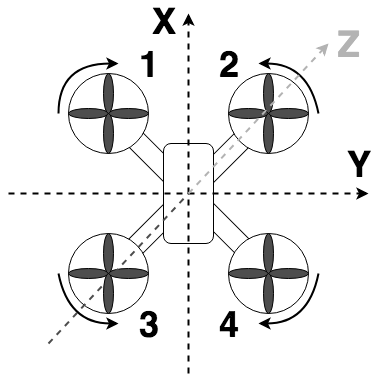
\includegraphics[scale=0.5]{drone.png}
        \caption{Scheme of the drone.}
    \end{figure}

    Body rate controller returns desired angular accelerations of the quadrotor. Altitude controller returns a collective thrust of a quadrotor, required to reach desired altitude taking current attitude of the quad into account. Our goal is to distribute this collective thrust between the propellers to reach the desired angular velocities.

    Propeller that rotates with angular velocity $\omega$ generates thrust
    \begin{equation*}
        F = k_f\omega^2
    \end{equation*}

    Total thrust generated by four propellers is a sum of thrusts generated by each propeller
    \begin{equation*}
        F_c = F_1+F_2+F_3+F_4
    \end{equation*}

    Moments produced by rotors are
    \begin{align*}
        \tau_1 &= -k_m\omega_1^2 \\
        \tau_2 &= k_m\omega_2^2 \\
        \tau_3 &= k_m\omega_3^2 \\
        \tau_4 &= -k_m\omega_4^2
    \end{align*}

    Take into account, that 1st and 4th rotors rotate clockwise and produce negative moments in counterclockwise direction, while 2nd and 3rd rotors rotate counterclockwise and produce positive moments.

    Moments produced by propellers around the $x$, $y$ and $z$ axes are:
    \begin{align*}
        \tau_x &= (F_1+F_3-F_2-F_4)l \\
        \tau_y &= (F_1+F_2-F_3-F_4)l \\
        \tau_z &= \tau_1+\tau_2+\tau_3+\tau_4
    \end{align*}

    Our controller returns the following inputs: collective thrust $F_C$ and angular accelerations $\bar{u}_p = \dot{p}$, $\bar{u}_q = \dot{q}$, $\bar{u}_r = \dot{r}$. We have to find the angular velocities of the propellers $\omega_1$, $\omega_2$, $\omega_3$, $\omega_4$.

    As we know, the acceleration $\alpha$ around the axis is proportional to the applied thrust and equals to $\alpha=\frac{\tau}{I}$, where $I$ is a moment of inertia around the axis. For our inputs accelerations may be written as:
    \begin{align*}
        \bar{u}_p &= \dot{p} = \frac{\tau_x}{I_x} = \frac{(F_1+F_3-F_2-F_4)l}{I_x} = \frac{(\omega_1^2+\omega_3^2-\omega_2^2-\omega_4^2)lk_f}{I_x} \\
        \bar{u}_q &= \dot{q} = \frac{\tau_y}{I_y} = \frac{(F_1+F_2-F_3-F_4)l}{I_y} = \frac{(\omega_1^2+\omega_2^2-\omega_3^2-\omega_4^2)lk_f}{I_y} \\
        \bar{u}_r &= \dot{r} = \frac{\tau_z}{I_z} = \frac{\tau_1+\tau_2+\tau_3+\tau_4}{I_z} = \frac{(-\omega_1^2+\omega_2^2+\omega_3^2-\omega_4^2)k_m}{I_z}
    \end{align*}

    Now we can convert this to dimensionless form:
    \begin{align*}
        \bar{c} &= \frac{F_c}{k_f} = \omega_1^2+\omega_2^2+\omega_3^2+\omega_4^2 \\
        \bar{p} &= \frac{I_x\bar{u}_p}{k_fl} = \omega_1^2+\omega_3^2-\omega_2^2-\omega_4^2 \\
        \bar{q} &= \frac{I_y\bar{u}_q}{k_fl} = \omega_1^2+\omega_2^2-\omega_3^2-\omega_4^2 \\
        \bar{r} &= \frac{I_z\bar{u}_r}{k_m} = -\omega_1^2+\omega_2^2+\omega_3^2-\omega_4^2
    \end{align*}

    And the only we have to do now is to find angular velocities of the propellers:
    \begin{align*}
        \omega_4^2 &= \frac{\bar{c}-\bar{p}-\bar{q}-\bar{r}}{4} \\
        \omega_3^2 &= \frac{\bar{c}-\bar{q}}{2} - \omega_4^2 \\
        \omega_2^2 &= \frac{\bar{c}-\bar{p}}{2} - \omega_4^2 \\
        \omega_1^2 &= \bar{c} - \omega_2^2 - \omega_3^2 - \omega_4^2
    \end{align*}

    Remember that counterclockwise rotation has negative velocity:
    \begin{align*}
        \omega_1 &= \sqrt{\omega_1^2} \\
        \omega_2 &= -\sqrt{\omega_2^2} \\
        \omega_3 &= -\sqrt{\omega_3^2} \\
        \omega_4 &= \sqrt{\omega_4^2}
    \end{align*}
\end{document}
